%%==================================================
%% chapter03.tex for SJTU Master Thesis
%% Encoding: UTF-8
%%==================================================

\chapter{混合现实眼镜下的空间交互设计}
\label{chap:interaction}

本章结合上一章设计的三维界面,设计本文系统的第二个部分:空间交互。
本文系统采用以手势交互为主结合其他辅助方式的交互方法。
先介绍本文系统所使用的三个手势的设计思想与实现细节,
然后本文系统根据第\ref{chap:exp}章阐述的可行性实验评估结果优化,设计了多项辅助方式,分别是顶置提示板、骨骼小球和头部约束帮助用户进行空间交互。



\section{三维界面上的手势设计与实现}
%\begin{figure}[!htp]
  %\centering
  %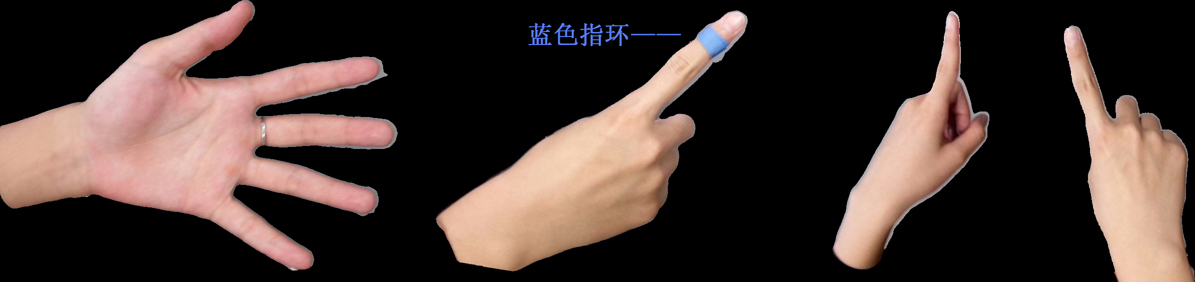
\includegraphics[width=0.6\textwidth]{chap4/gesture}
  %\bicaption[fig:gestures]{三种手势}{三种手势}{Fig.}{Three gestures}
%\end{figure}

\begin{figure}[!htp]
	\centering
	\subfigure{\label{fig:gestures:menu}}\addtocounter{subfigure}{-2}
	\subfigure[Menu gesture]{\subfigure[菜单手势]
		{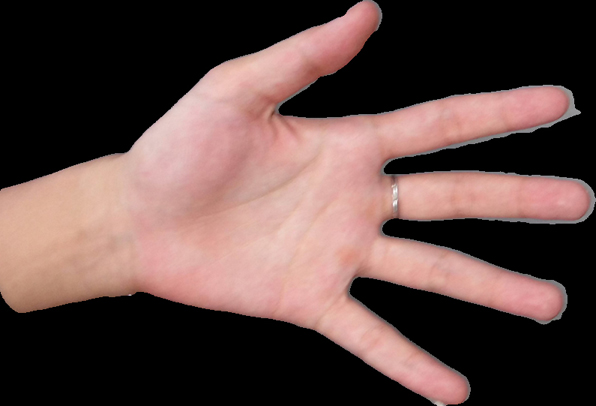
\includegraphics[width=0.32\textwidth]{chap4/gesture-menu}}}
	\subfigure{\label{fig:gestureselect}}\addtocounter{subfigure}{-2}
	\subfigure[Selection gesture]{\subfigure[选择手势]
		{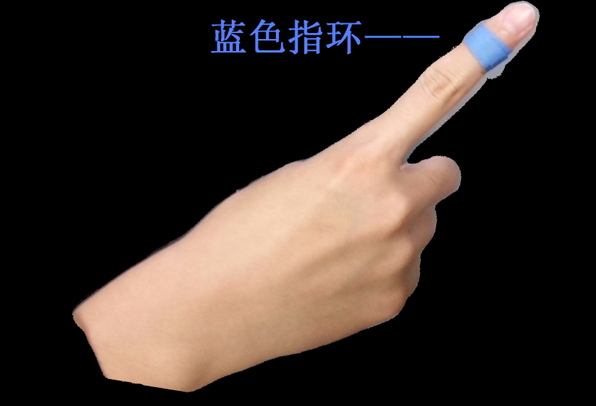
\includegraphics[width=0.32\textwidth]{chap4/gesture-select}}}
		\subfigure{\label{fig:gesture:manipulate}}\addtocounter{subfigure}{-2}
	\subfigure[Manipulation gesture]{\subfigure[操控手势]
		{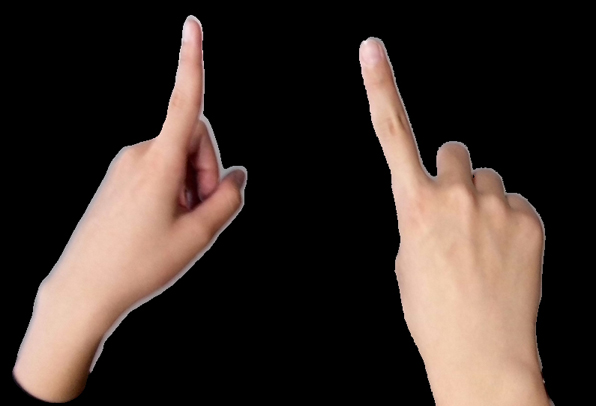
\includegraphics[width=0.32\textwidth]{chap4/gesture-mani}}}
	\bicaption[fig:gestures]{三种手势}{三种手势}{Fig.}{Three gestures}
	%\bicaption[总标签名]{}{中文总标题}{Fig.$\!$}{The total caption}
	\vspace{-1em}
\end{figure}

由\ref{sec:design-principle}节提到的设计原则,本文系统一共设计了三个手势:菜单手势、选择手势和操控手势。
由图\ref{fig:gestures}(a)可见,菜单手势即五指自然张开,本文系统检测到时便会将手掌召唤式菜单安置在掌心位置。
由图\ref{fig:gestures}(b)所示,选择手势使用色环触发,另一只手的手指戴上一个蓝色色环后,本文系统进入选择模式,如图\ref{fig:logicRelationship}所示,此刻无论是召唤菜单或者操控物体都不能进行,只能进行对菜单或者物体的选择。
当手指悬停选中菜单一定时间后,菜单消失表示指令已被选中。
根据所选的菜单选项,使用单手或双手进行操控,每只手自然伸出一根手指如图\ref{fig:gestures}(c)所示,即可对当前被选中的物体们进行操控。

本文中提到的操控是物体的几种基本操控:平移,旋转和缩放。

\begin{figure}[!htp]
  \centering
  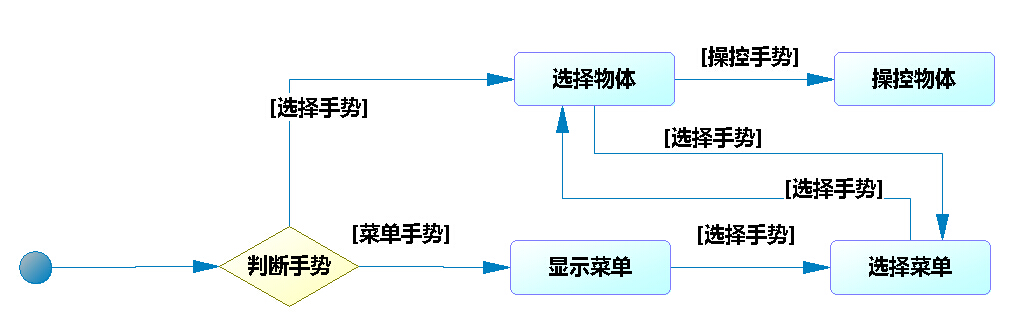
\includegraphics[width=0.95\textwidth]{chap4/gestureLogic}
  \bicaption[fig:logicRelationship]{三种手势的逻辑关系图}{三种手势的逻辑关系图}{Fig.}{the logic relationship among three gestures}
\end{figure}

\subsection{菜单手势}

菜单手势针对手掌召唤式菜单所设计,由USB相机输入的图像和Leap Motion输入的图像结合分析。
通过手指检测算法先判断USB相机的输入图像中是否有肤色区域内含五根手指,为了增加容错率,本文系统后期改为检测至少四根手指。
另一方面从Leap Motion处获得手部骨架,两处输入同时判断:是否同为左手或右手,如果不是,本文系统将当前手势信息状态置空;自然伸出的手指数量是否一致,
如果数量不一致则不继续;在两个输入一致通过检测后,本文系统利用先前粗略进行的Leap Motion和相机标定结果在手掌对应的位置绘制出调色盘菜单。
由于相机输入受环境影响颇大,此处对相机丢失信号的容忍度设了一个阈值T,只要在连续T帧内重新识别到手势,本文系统就继续显示调色盘菜单,反之则消失。

菜单手势实现算法如算法\ref{alg:menu}所示,先进行左右眼图像的立体匹配而后获取肤色区域,然后通过开操作和闭操作的降噪后获取最大的轮廓来进行判断是否有手指的存在。
	\begin{algorithm}  
		\caption{菜单手势实现算法}  
		\label{alg:menu} 
		\begin{algorithmic}  
		\REQUIRE{左右眼的两幅输入图像$Image_l_e_f_t$和$Image_r_i_g_h_t$}
		\ENSURE{手势类型$GestureType$和手指数据$HandInfo$}
			\STATE {对$Image_l_e_f_t$和$Image_r_i_g_h_t$进行立体匹配,校正图像}
			%\STATE {对左右眼的两幅输入图像进行色环提取}
			\STATE {对$Image_l_e_f_t$和$Image_r_i_g_h_t$进行肤色区域提取,为$Skin_l_e_f_t$和$Skin_r_i_g_h_t$}
			\FOR{each $image \in [Skin_l_e_f_t,Skin_r_i_g_h_t]$}
				\STATE {对$image$进行开闭等形态学降噪,为$image_i_m_p$}
				\STATE {获取$image_i_m_p$最大的两个轮廓$Hole_f$和$hole_s$}
				\FOR{each $hole \in [Hole_f,hole_s]$}
					\STATE {对$hole$多边形拟合进行手指识别,设置手指数据,手指数量记为$n$}
				\ENDFOR
				\IF{$n >= 4$}
					\STATE {$GestureType=MENU$}
					\STATE{填充$HandInfo$}
				\ENDIF
			\ENDFOR			
		\end{algorithmic}  
	\end{algorithm} 
\subsection{选择手势}

%\begin{description}
%\item[选择手势设计思想]\hfill\\
选择手势采用最常用的单手食指动作,模拟鼠标的左键,通常也是最常见的点击与选中意义。
然而如\ref{sec:input}节所提Leap Motion与相机间的粗略标定,当精确到需要提取用户指尖位置的时候,误差偏大因而这里采用了色环作为辅助工具。
色环颜色采用与肤色呈反色的蓝色调,简单易制作且轻量级几乎对用户没有任何压力。
同时自然地分割了移动与选中的状态切换。
当用户想要选中物体时,需佩戴上色环,此时摄像头捕捉到色环便默认用户正在进行选择,选择菜单或者选择目标物。
当摄像头没有捕捉到色环时,则对用户的手指移动进行操控手势的理解。

%\item[选择手势实现算法]\hfill\\
算法\ref{alg:select}详述了选择手势算法的实现。
其一考虑容错率,因而在转换成HSV空间的图像中对蓝色掉提取时放宽约束,捕获到场景内所有接近蓝色调的物体。
然后进行形态学闭操作,并根据区域大小大小过滤掉不符合要求的蓝色区域。
接着遍历所有候选者,与同时期获得的肤色区域进行闭操作。此时由于蓝色指环导致食指的肤色区域被分为两个部分,如果该候选者即色环区域,则这三个区域可以合并成为一根手指。
以关操作后是否成为一个连通域作为判断标准来寻找色环,增加了其稳定性。
而色环的位置也就是之后用户表示选中的位置。
由图\ref{fig:colorRing}可观察选择手势识别中的每一步的处理过程与结果展示

\begin{figure}[!htp]
	\centering
	\subfigure{\label{fig:colorRing:a}}\addtocounter{subfigure}{-2}
	\subfigure[Input image]{\subfigure[输入图像]
		{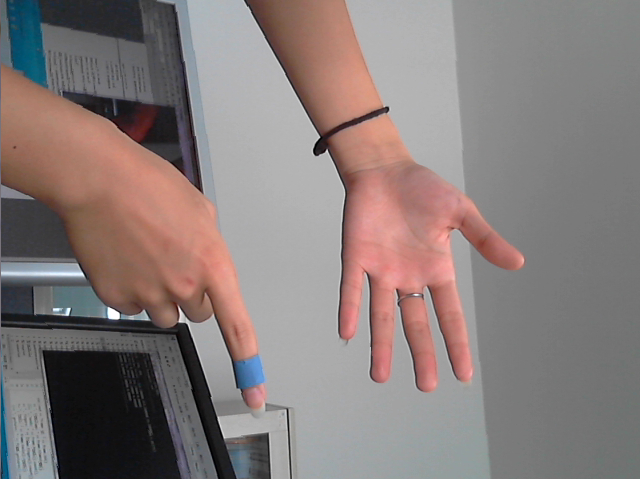
\includegraphics[width=0.3\textwidth]{chap4/color1}}}
	\subfigure{\label{fig:colorRing:b}}\addtocounter{subfigure}{-2}
	\subfigure[HSV color space]{\subfigure[HSV色彩空间]
		{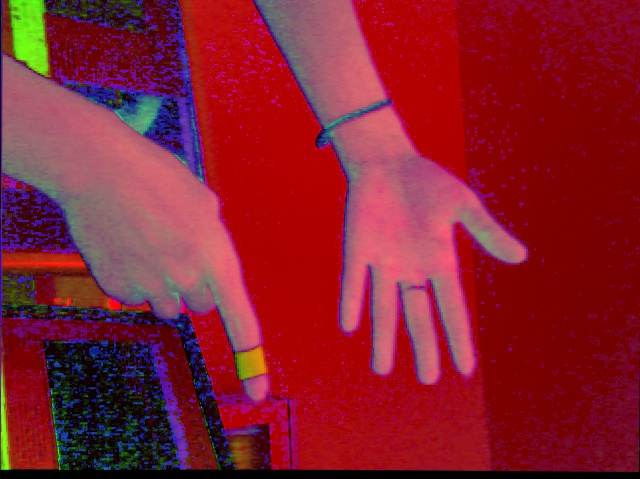
\includegraphics[width=0.3\textwidth]{chap4/color2-hsv}}}
	\subfigure{\label{fig:colorRing:c}}\addtocounter{subfigure}{-2}
	\subfigure[Skin extraction]{\subfigure[肤色提取]
		{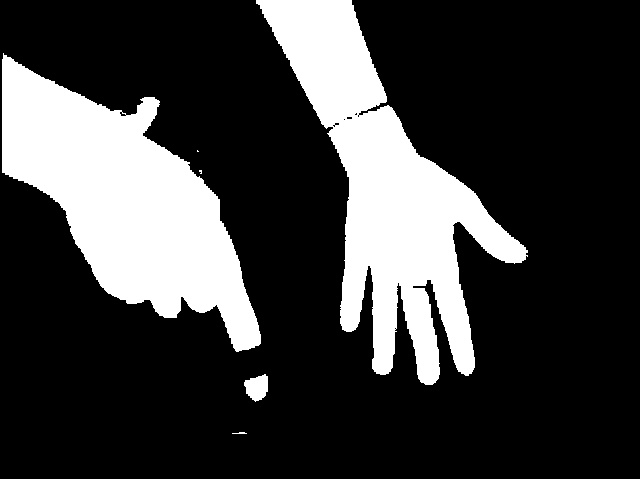
\includegraphics[width=0.3\textwidth]{chap4/color3-skin}}}
	\vspace{-1em}
	\subfigure{\label{fig:colorRing:menu}}\addtocounter{subfigure}{-2}
	\subfigure[Color ring extraction]{\subfigure[色环提取]
		{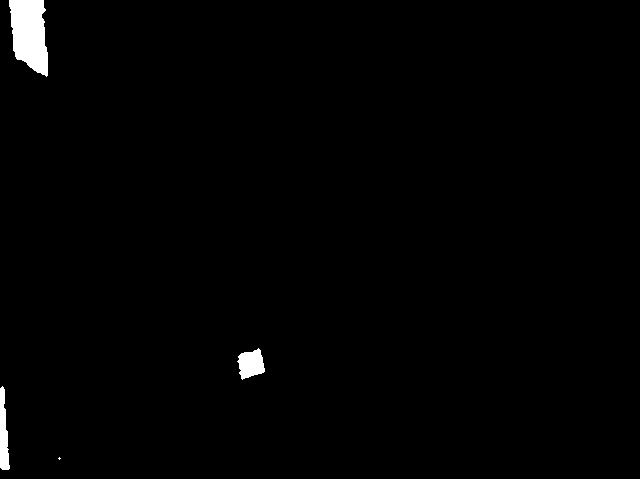
\includegraphics[width=0.3\textwidth]{chap4/color4-blue}}}
	\subfigure{\label{fig:colorRing:e}}\addtocounter{subfigure}{-2}
	\subfigure[Close operation]{\subfigure[闭操作]
		{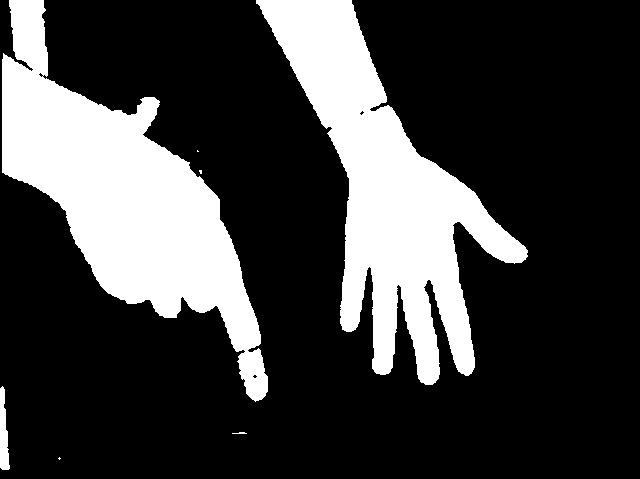
\includegraphics[width=0.3\textwidth]{chap4/color5-close}}}
	\subfigure{\label{fig:colorRing:f}}\addtocounter{subfigure}{-2}
	\subfigure[Mark color ring]{\subfigure[标记色环]
		{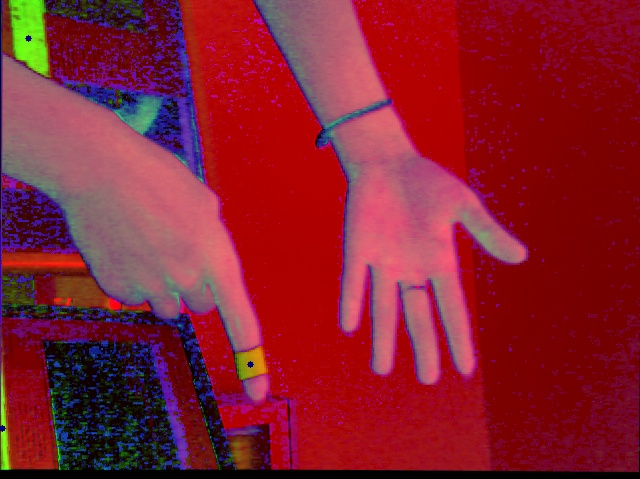
\includegraphics[width=0.3\textwidth]{chap4/color6-circle}}}
	\bicaption[fig:colorRing]{色环的处理过程}{色环的处理过程}{Fig.}{Process for color ring}
	%\bicaption[总标签名]{}{中文总标题}{Fig.$\!$}{The total caption}
	\vspace{-1em}
\end{figure}
	\begin{algorithm}  
		\caption{选择手势实现算法}  
		\label{alg:select} 
		\begin{algorithmic}
\REQUIRE{左右眼的两幅输入图像$Image_l_e_f_t$和$Image_r_i_g_h_t$}
\ENSURE{手势类型$GestureType$和手指数据$HandInfo$}
			\STATE {对$Image_l_e_f_t$和$Image_r_i_g_h_t$进行立体匹配,校正图像}
			\STATE {对$Image_l_e_f_t$和$Image_r_i_g_h_t$进行色环提取,记录$n$个候选色环点$circle_c_a_n_d$}
			\FOR{each $circle \in circle_c_a_n_d$}
				\IF{检测到色环}
					\STATE {对$Image_l_e_f_t$和$Image_r_i_g_h_t$进行肤色区域提取,为$Skin_l_e_f_t$和$Skin_r_i_g_h_t$}
					\FOR{each $skin \in [Skin_l_e_f_t,Skin_r_i_g_h_t]$}
						\STATE {对$skin$采用形态学开闭操作进行降噪,为$skin_i_m_p$}
						\STATE {获取$skin_i_m_p$最大的两个轮廓,为$contour_f$和$contour_s$}
						\FOR{each $contour \in [contour_f,contour_s]$}
							\STATE {将$contour$与色环候选区域合并}
							\STATE {形态学处理得到最大的轮廓$contour_m_a_x$}
							\FOR{each $i \in [1,n]$}
								\IF{判断候选点是否在轮廓范围内}
									\STATE{$GestureType=SELECT$}
									\STATE{填充$HandInfo$}
								\ENDIF
							\ENDFOR
							\STATE{如果均无则$GestureType=NULL$}
						\ENDFOR
					\ENDFOR	
				\ENDFOR
			\ELSE
				\STATE {$GestureType=NULL$}
			\ENDIF
		\end{algorithmic}  
	\end{algorithm} 

%\end{description}

%\begin{figure}[!htp]
  %\centering
  %\includegraphics[width=0.6\textwidth]{chap4/testpng}
  %\bicaption[fig:colorRing]{色环的处理过程}{色环的处理过程}{Fig.}{process for color ring}
%\end{figure}

\subsection{操控手势}

%\begin{description}
%\item[操控手势设计思想]\hfill\\
%\subsubsection{操控手势设计思想}
操控手势的设计思想在于操控手势不论单手双手都是用户自然伸直食指进行操控的。
区别在于具体的操控逻辑。
%\item[单手操控实现算法]\hfill\\
\subsubsection{单手操控实现算法}

单手操控时,首先选择具体指令。
如果是平移:平移的位移与手的位移一致,基本上就是直接对应的操作;
如果是旋转:旋转角度由手的移动距离决定,移动的距离越大则转的角度越多,而旋转轴由手的移动轨迹决定,基本和触摸屏操控一致,只不过没有固定触摸屏的限制于是用户可以进行譬如Z轴方向的移动;
如果是缩放,则根据常识向右向上向前为放大,反之为缩小,而缩放的幅度由手的位移决定。
%\item[双手操控实现算法]\hfill\\
\subsubsection{双手操控实现算法}

\begin{algorithm}  
		\caption{双手操控实现算法}  
		\label{alg:double} 
		\begin{algorithmic}  
		\REQUIRE{左右双手$Hand_l_e_f_t$和$Hand_r_i_g_h_t$,手的类型$HandType$,操控之手数量$m$,左右双手位置$pos_l_e_f_t$和$pos_r_i_g_h_t$,左右双手上一帧的位置$posPre_l_e_f_t$和$posPre_r_i_g_h_t$}
		\ENSURE{变换类型$TransType$和参数数组$para$}
		\STATE {$m=0$}
		\FOR{each $hand \in [Hand_l_e_f_t,Hand_r_i_g_h_t]$}
			\FOR{each $fingerIdx \in [1,5]$}
				\IF {手指自然伸直}
					\STATE {手指数量$n=n+1$}
				\ENDIF
			\ENDFOR
			\IF{$n == 1$}
				\STATE{$hand.HandType = MNPL$}
				\STATE {$m=m+1$}
			\ENDIF
		\ENDFOR
		\IF{$m == 2$}
			\STATE{$vec_c_u_r = pos_l_e_f_t-pos_r_i_g_h_t$}
			\STATE{$vec_p_r_e = posPre_l_e_f_t-posPre_r_i_g_h_t$}
			\STATE{$vec_l_e_f_t = pos_l_e_f_t-posPre_l_e_f_t$}
			\STATE{$vec_r_i_g_h_t = pos_r_i_g_h_t-posPre_r_i_g_h_t$}
			\STATE{$rotateAngle = angle(vec_c_u_r,vec_p_r_e)$}
			\IF{$rotateAngle <= \pi/9$}
				\STATE{$TransType = TRANS$}
				\STATE{$para[0] = (vec_l_e_f_t + vec_r_i_g_h_t) / 2$}
			\ELSIF{$rotateAgle >= \pi*5/6$}
				\STATE{$TransType = SCALE$}
				\STATE{$para[0] = vec_c_u_r / vec_p_r_e$}
			\ELSIF{$rotateAngle \in [\pi/6,\pi/2]$}
				\STATE{$TransType = ROTATE$}
				\STATE{$para[0] = cross(vec_l_e_f_t,vec_r_i_g_h_t)$}
				\STATE{$para[1] = rotateAngle$}
			\ENDIF
		\ENDIF
	\end{algorithmic}  
\end{algorithm} 
	
双手操控时,本文系统会同时判断是否在进行平移、旋转,和缩放,用户可以同时进行这些操控,具体算法见算法\ref{alg:double}。
本文系统对两只手的位移进行分析,分离两只手在X轴、Y轴和Z轴三轴上的矢量,如果在同一轴上的矢量是同向的,则取其均值作为平移参数,将符合条件的矢量相加得到最后的平移指令;
如果分离出是相向运动,则进行放缩,放缩的参数由该方向的移动后距离与移动前距离做比值,以该比值为参数调整目标物体的大小;
然后对左手和右手的移动路径做叉乘,看是否存在扭矩。
存在则以叉乘结果矢量为旋转轴,结果绝对值为旋转角度参数。
双手操控由于可以同时进行三种基本变换,因而省略了切换命令的步骤,并且同时发出多个指令也是的操控更为高效。
%\end{description}

\section{三维界面上的辅助设计}

在易用性用户实验后,根据用户的反馈与提议,本文所设计的系统增加了其他的辅助功能帮助用户更好地体验这一套三维菜单和三维操控手势。
以下为新增的辅助设计。

\subsection{顶置提示板}
\label{fig:interaction:board}
%\begin{figure}[!htp]
  %\centering
  %\includegraphics[width=0.3\textwidth]{chap4/testpng}
  %\hspace{1cm}
  %\includegraphics[width=0.3\textwidth]{chap4/testpng}
  %\bicaption[fig:board]{顶置提示板}{顶置提示板}{Fig.}{Board}
%\end{figure}
根据实验反馈,我们得到使当前系统状态更明朗化的提议,于是在用户视野的正上方显示了一个提示板,提示当前用户正在进行的操作,安置在正上方是为了让提示板的存在不影响到整体布局。
随着用户的操作,提示板的内容会因之变化,关于其布局位置与是否有存在价值将会在之后的实验具体说明。

\subsection{骨骼小球}
\label{sec:interaction:skeleton}
%\begin{figure}[!htp]
  %\centering
  %\includegraphics[width=0.4\textwidth]{chap4/skeletonball1}
  %\hspace{1cm}
  %\includegraphics[width=0.4\textwidth]{chap4/skeletonball2}
  %\bicaption[fig:skeletonball]{骨骼小球}{骨骼小球}{Fig.}{skeletonball}
%\end{figure}

另一修改点是关于Leap Motion。对不少实验者而言,Leap Motion也是一个全新的设备,并没有任何使用过的经验,于是实验中除了新增熟悉Leap Motion的步骤外,对于其在实验进行中的可视化也是一个辅助用户操作的办法。
这里的设计是增加了骨骼小球,而骨骼小球的位置与用户的手一一对应,用户可以通过观察骨骼小球的位置得知目前自己的手在Leap Motion系统中是什么情况,以及是否被正确识别。
因为最初的实验中经常遇到本文系统未对用户的操控进行响应的情况,而其原因大部分是Leap Motion并未捕捉到用户的手。
虽然Leap Motion和人眼的物理位置非常接近,但其视角的不同导致用户所见的场景并不是Leap Motion所见,于是骨骼小球的存在就可以用于提示用户。

\begin{figure}[!htp]
	\centering
	\subfigure{\label{fig:skeletonball:a}}\addtocounter{subfigure}{-2}
	\subfigure[Selection gesture with skeleton ball]{\subfigure[选择手势下的骨骼小球]
		{\includegraphics[width=0.4\textwidth]{chap4/skeletonball1}}}
	\subfigure{\label{fig:skeletonball:b}}\addtocounter{subfigure}{-2}
	\subfigure[Menu gesture with selection gesture]{\subfigure[菜单手势下的骨骼小球]
		{\includegraphics[width=0.4\textwidth]{chap4/skeletonball2}}}
	\bicaption[fig:skeletonball]{骨骼小球}{骨骼小球}{Fig.}{Skeleton ball}
	%\bicaption[总标签名]{}{中文总标题}{Fig.$\!$}{The total caption}
	\vspace{-1em}
\end{figure}

如图\ref{fig:skeletonball}所示,相同颜色的骨骼小球表示相同的手指,如果视野中未出现一个骨骼小球,表示当前检测不到任何有效的手。
通过观察骨骼小球,用户可以调整自己的手势来更好地操控。
对于骨骼小球布局及存在价值,会在进一步的实验中详细验证。

\subsection{头部约束}
\label{sec:interaction:head}
头部约束的想法来源与手掌召唤式菜单,手掌召唤式菜单的动作与其说是显示自己的手心,更接近一个翻转手腕的动作,而这个动作通常以低头完成更加自然。
于是针对部分用户反馈的菜单过于容易被触发的问题,改进后的系统中增加了对手掌召唤式菜单的头部约束,模拟画家画画时的景象,选用调色盘上的颜
料时,总是低头看向捧着的调色盘。于是改进后的系统中约束用户只有在低头的时候才能触发该菜单,一方面避免了菜单无意中被触发的情况,另一方面帮助
用户将菜单操作区域和虚拟物体操作区域划分得更清楚,减少无意中选中物体的情况。

\begin{figure}[!hpb]
	\centering
	\subfigure{\label{fig:threeaction:a}}\addtocounter{subfigure}{-2}
	\subfigure[Menu gesture of user]{\subfigure[真人菜单手势]
		{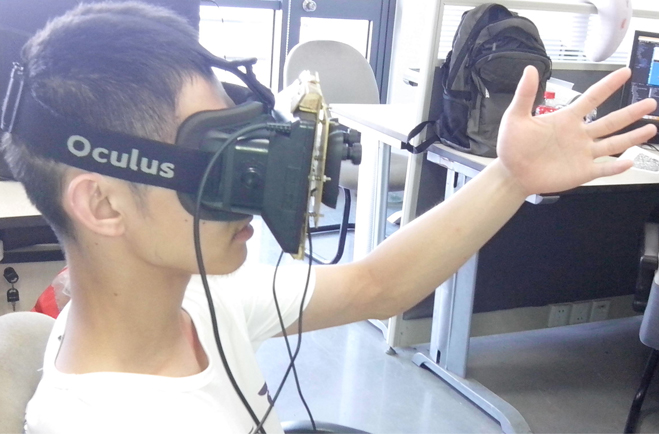
\includegraphics[height=0.2\textheight]{chap4/three-action-l1}}}
	\subfigure{\label{fig:threeaction:b}}\addtocounter{subfigure}{-2}
	\subfigure[Menu gesture in ARGlasses]{\subfigure[场景菜单手势]
		{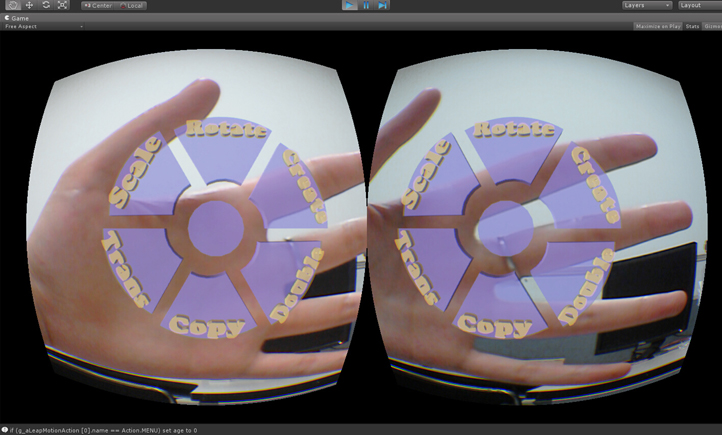
\includegraphics[height=0.2\textheight]{chap4/three-action-r1}}}
	\vspace{-1em}
	
	\subfigure{\label{fig:threeaction:c}}\addtocounter{subfigure}{-2}
	\subfigure[Selection gesture of user]{\subfigure[真人选择手势]
		{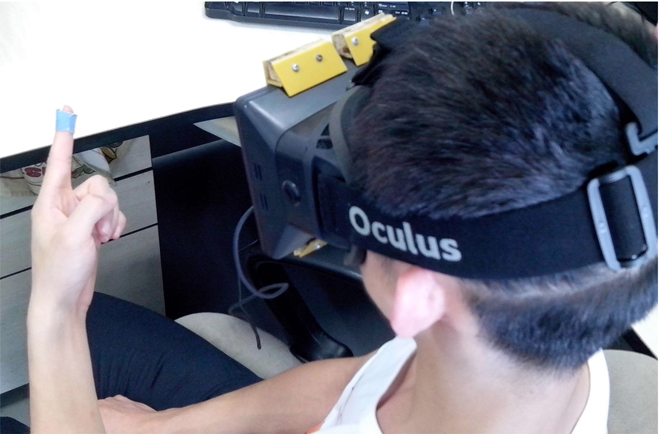
\includegraphics[height=0.2\textheight]{chap4/three-action-l2}}}	
	\subfigure{\label{fig:threeaction:menu}}\addtocounter{subfigure}{-2}
	\subfigure[Selection gesture in ARGlasses]{\subfigure[场景选择手势]
		{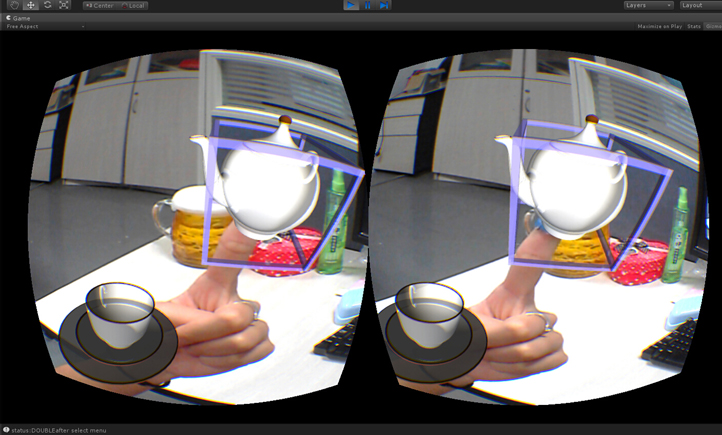
\includegraphics[height=0.2\textheight]{chap4/three-action-r2}}}
	\vspace{-1em}
	
	\subfigure{\label{fig:threeaction:e}}\addtocounter{subfigure}{-2}
	\subfigure[Manipulation gesture of user]{\subfigure[真人操控手势]
		{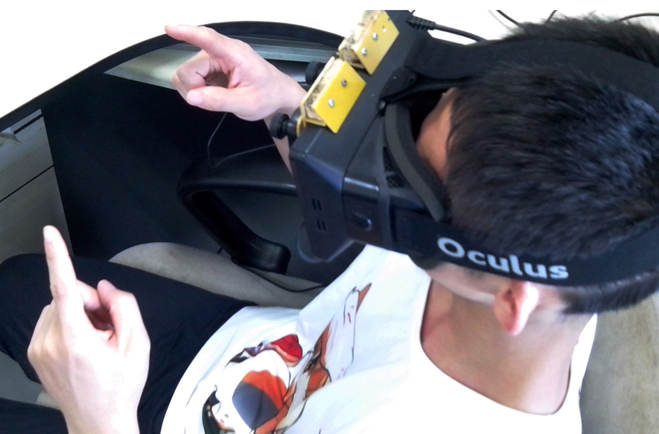
\includegraphics[height=0.2\textheight]{chap4/three-action-l3}}}
	\subfigure{\label{fig:threeaction:f}}\addtocounter{subfigure}{-2}
	\subfigure[Manipulation gesture in ARGlasses]{\subfigure[场景操控手势]
		{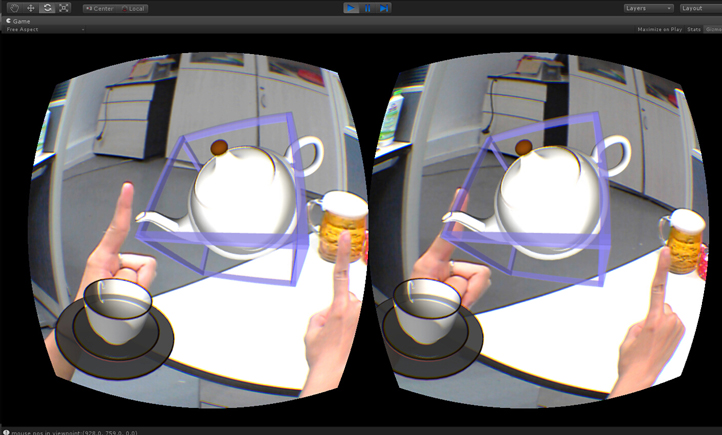
\includegraphics[height=0.2\textheight]{chap4/three-action-r3}}}
	\bicaption[fig:threeaction]{手势实景一览}{手势实景一览}{Fig.}{Three gestures in real scene}
	\vspace{-1em}
\end{figure}

\section{本章小结}
本章承接前一章的设计原则设计了用户在混合现实眼镜下的交互方式。出于学习与记忆的考虑,本文系统一共设计如图所示\ref{fig:threeaction}三个手势:菜单手势、选择手势和操控手势。
并简要介绍每个手势的设计思想和实现方法。
菜单手势由画家与调色盘的寓意而来。
选择手势沿用最通用的点击姿势,并由于硬件设备当时的融合原因增加了色环的设计,同时结合色环的设计配合\ref{sec:related-zhuangtai}节提到的状态切换的考虑,设计了选择手势与其他手势间的逻辑。
操控手势分成单双手分别介绍其交互细节与实现算法。
而后列举了在实验评估后增补的修改设计,分别是用于提醒用户当前指令的顶置提示板,提示用户手部骨骼的骨骼小球和配合手掌召唤式菜单用于工作空间分离减少误操作的头部约束。而对所有的交互设计都将在第\ref{chap:exp}章中详细评估。